\documentclass[a4paper]{IEEEtran}

\usepackage{xcolor}
\usepackage{hyperref}
\usepackage[utf8]{inputenc}
\usepackage[pdftex]{graphicx} 
\usepackage{multirow, pgfplotstable,booktabs,colortbl,lmodern}

\newcommand\TODO[1]{\textcolor{red}{TODO:#1}}
\newcommand\todo[1]{\TODO{#1}}
\newcommand\cn{\textcolor{red}{[citation needed]}}

\title{The overpowered prefetcher of goodness and excellence!}

\author{
    Sigve Sebastian Farstad,
    Rune Holmgren,
    Torbjørn Langland,
    Per Thomas Lundal
}

\begin{document}

\maketitle

\begin{abstract}
    Le abstract.\cn
\end{abstract}

\section{Introduction}

\todo{ Write briefly about the project, the course it belongs to and the goal}
This is the introduction section.
Here we write something appealing for you to continue on.
If you finish this, you will be baked a cake.

As part of the course TDT4260 Computer Architecture, students in groups of 3 or 4 were to implement and test a prefetcher.
This report describes the implementation with test results done by group 11.
The report will describe the framework for the project, different prefetchers that have been implemented, how they work and the test results.

\section{Related Work}

\todo{ Not sure, mention related work?}
Here we mention related work. Do you want cake for your relatives?

\subsection{Delta Correlation Prefetching}
\todo{write something!}

\subsection{Global History Buffer}
History based prefetchers need to store access patterns efficient data structure that enables quick access.
One such data structure is the Global History Buffer (GHB) \cite{ghb}.
GHB is an $n$-entry First-In, First-Out (FIFO) queue implemented as a circular buffer.
It stores the $n$ most recent L1 cache misses in entries that contain the miss address and a link pointer.
The link pointer is used to chain entries together into time-ordered linked lists that holds the significant access patterns.
An Index Table (IT) is used to keep track of these lists.
It maps some key to the most recent element of a linked list.
The IT is based on a FIFO queue like GHB, but significantly smaller as each entry has to be evaluated for each cache miss to look up a matching key.
The key can be based on any cache miss information, and depending on it a wide variety of history based prefetch methods can be implemented.
In a comparison of different prefetch mechanisms by Péres et al.\cite{microlib}, one using GHB gave the best performance.
\todo{figure}

\section{Prefetcher Description}
A total of 5 different prefetchers have been implemented and tested. 

\subsection{CZone Delta Correlation}
In this section, CZone Delta Correlation will be explained.

\begin{figure}[h!]
  \centering
      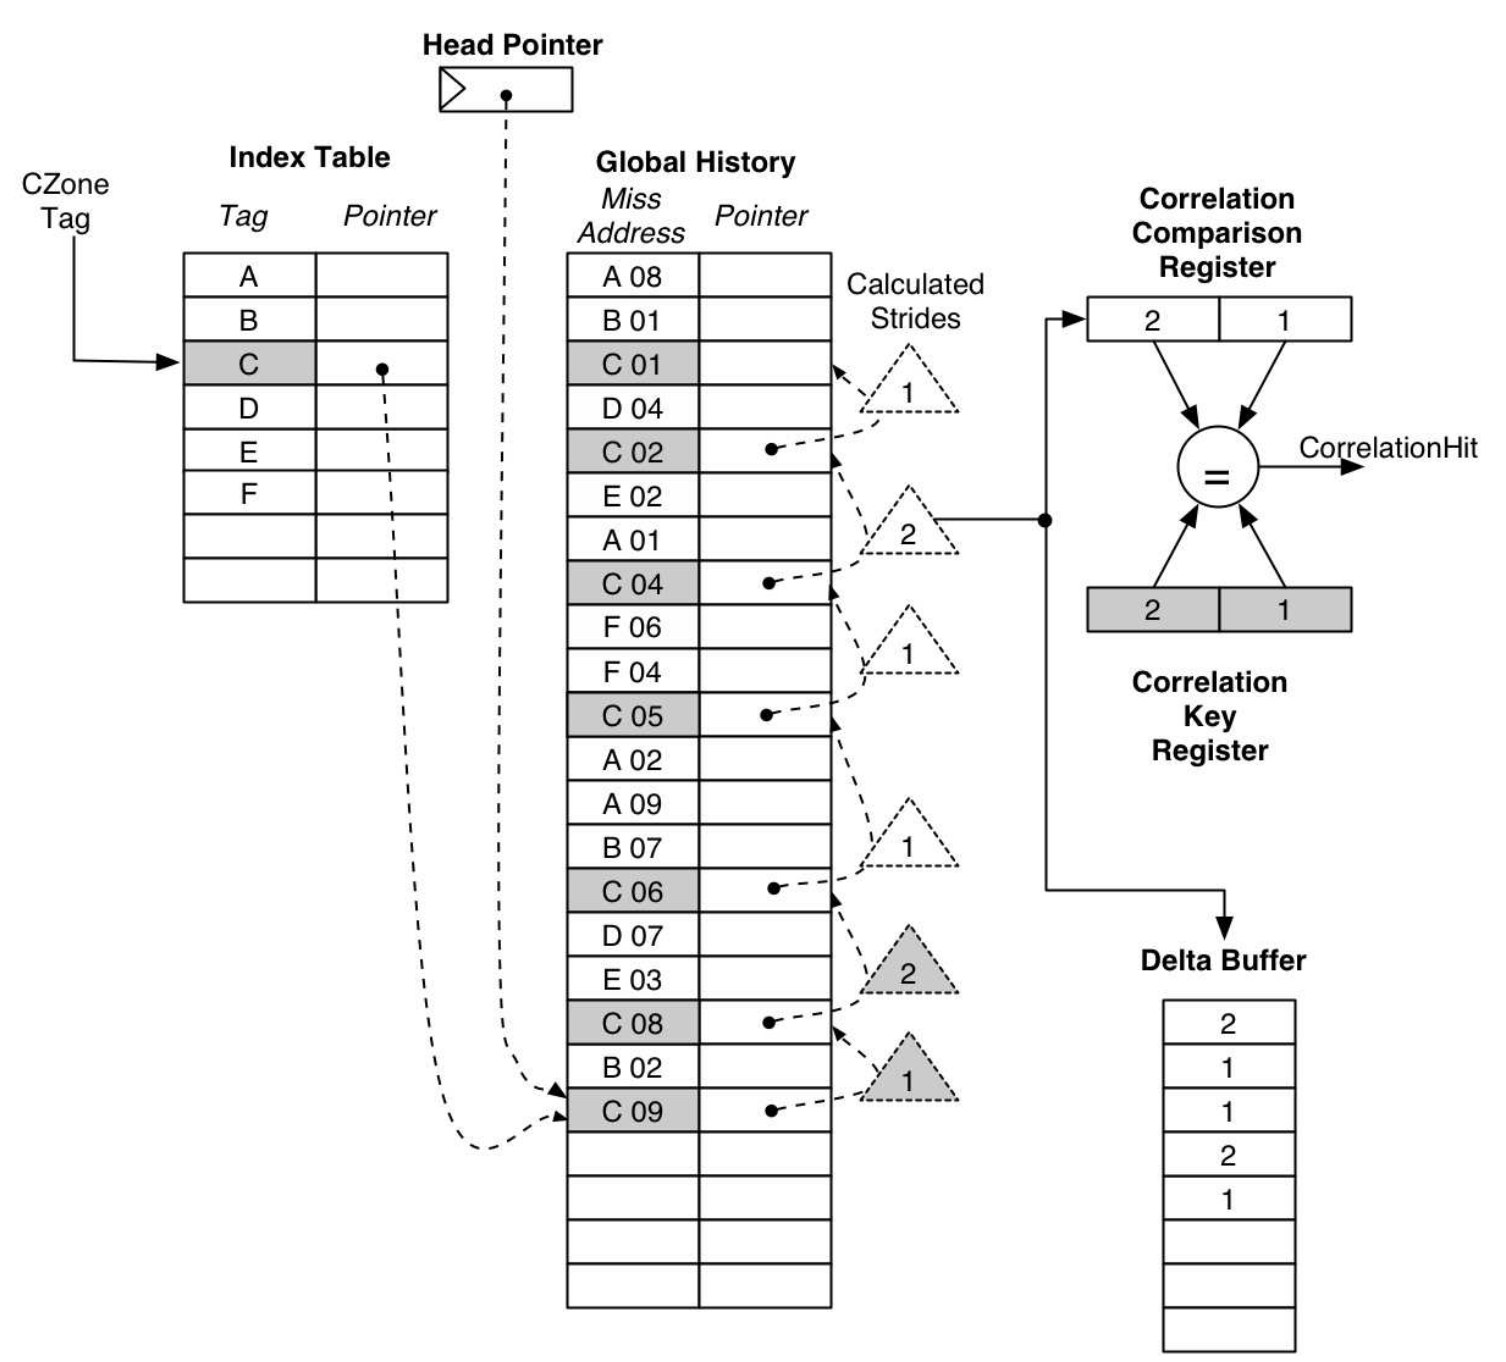
\includegraphics[width=0.5\textwidth]{Figures/CDC}
  \caption{CZone Delta Correlation Prefetch}
  \label{fig:CDC}
\end{figure}

Figure \ref{fig:CDC} shows how CZone Delta Correlation works. 
The memory is divided into different concentration zones (CZones). 
The different CZones that are accessed are put into an index table, with a tag of each CZone used for indexing, and a pointer to a Global History Buffer (GHB) that contains addresses for missed loads. 
In other types of prefetchers, these missed addresses are indexed in the GHB by the value of the PC, but in this case addresses from the same CZone are linked together using linked list, with the latest missed address entry as head. 
In the example figure, address C09 from CZone C is the head, and is linked to C08,  which again is linked to C06, etc. 
The pointers from the Index Table points to these heads.
The delta between the different addresses are calculated, and the first two from the linked list is added to the Correlation Key Register (2 and 1 in the example). 
The list is traversed, and the Correlation Comparison Register is continiously uptdated with the two latest deltas. 
Whenever there is a hit between the Comparison Registers and the Key Registers, and the distance between the current deltas and first two deltas in the linked list are not too great (max 2 in our implementation) a prefetch occurs. 
All deltas in between are added to a Delta Buffer, and they are used to calculate addresses for prefetch, using the two first addresses in the linked list and the contents in the delta buffer. 
The point with using CZones is that memory load patterns from different areas of the memory may be different of each other, and the idea is to calculate correct prefetch for the different memory loading patterns of the CZones.

\todo{ Figure \ref{fig:CDC} is picked from the internet. Add reference? }

\subsection{Adaptive CZone Delta Correlation}
The Adaptive CZone Delta Correlation Prefetcher is a more advanced version of the prefetcher described in previous subchapter.
While the non-adaptive version prefetches a static number of data blocks, this one dynamically calculates how many data blocks to prefetch.
The prefetcher increases or decreases the number of blocks to be prefetched by 1, after evaluating the hit rate.
The hit rate is compared with the hit rate of the previous setting, and the prefetcher increases or decreases the number of blocks based on increased or decreased performance. 

\subsection{Program Counter Delta Corelation}
\todo{write something}

\subsection{Adaptive Program Counter Delta Corelation}
\todo{write something}

\subsection{Delta Correlation Prediction Tables}

\todo{Describe how the final prefetcher works. I suggest adding a figure. Maybe briefly mention other attempts while if we have space?}

It is common for programs to access datastructures in neatly organized patterns.
In figure \ref{fig:DCExample} values are read with delta values 1 and 9, and this pattern repeats.
Such pattern may be exploited by prefetchers to predict what data will be read next.
A delta correlation prediction table will identify these patterns by comparing the delta values observed on misses with the history for resent misses.
When such patterns are found, the prefetcher will fetch the predicted cachelines into a circular buffer.


\begin{figure}[h!]
  \centering
      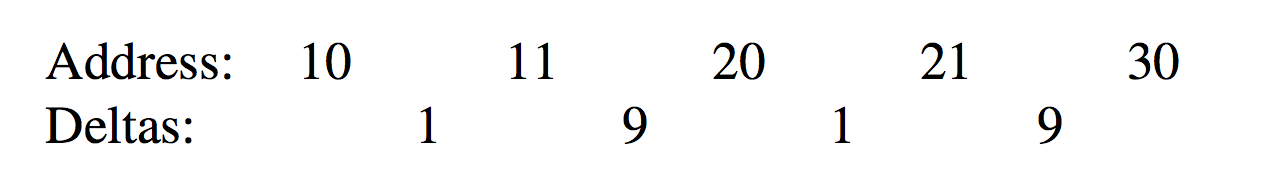
\includegraphics[width=0.5\textwidth]{Figures/DCExample}
  \caption{Delta Correlation Example}
  \label{fig:DCExample}
\end{figure}

As can be seen, the a row in the table contains fields for the PC, last address, last prefetch, deltas 1 to n, and delta pointer.
PC stores the address to the load instruction, and works as index in the table.
The Last Address stores the missed address when there is a miss in the cache.
The delta fields stores the address difference, or the deltas, for each time this instruction is called.
Last prefetch contains the address of the last issued prefetch.
The Delta Pointer points to the head (first Delta field) in the row, since the delta fields are used as circular buffer.

\begin{figure}[h!]
  \centering
      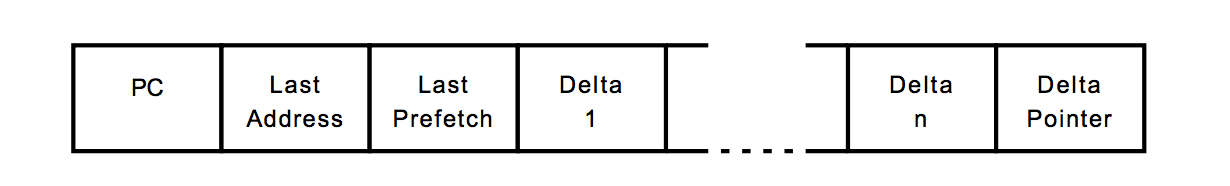
\includegraphics[width=0.5\textwidth]{Figures/DCTable}
  \caption{Delta Correlation Prediction Table}
  \label{fig:DCTable}
\end{figure}

\section{Methodology}

\todo{Mention the framework. Explain PFJudge. Maybe or maybe not mention C++?}
Here we describe how we did it.

WARNING: Recipee too long. Insert cake recipe here!

\section{Results}

\todo{ Describe results from both local and PFJudge.}

\pgfplotstableread{
test_name        dcpt  apcdc cdc pcdc 
{ammp}           1.478 1.501 1   1
{applu}          1.088 1.077 1   1
{apsi}           1.037 1.010 1   1
{art110}         1.042 1.058 1   1
{art470}         1.042 1.058 1   1
{bzip2\_graphic} 1.145 1.067 1   1
{bzip2\_program} 1.035 1.040 1   1
{bzip2\_source}  1.004 1.006 1   1
{galgel}         1.040 1.082 1   1
{swim}           1.031 1.035 1   1
{twolf}          0.992 0.991 1   1
{wupwise}        1.226 1.238 1   1
}\speeduptable

\newcommand{\mgraph}[2]{
\begin{tikzpicture}[scale=0.5]
\begin{axis}[
  ybar, bar width=1pt,ymin=0,
  xmin=0.5,xmax=12.5, xtick=data,
  %axis y discontinuity=crunch,
  %ymin=0.75,
  xticklabels from table={#1}{test_name},
  xticklabel style={rotate=45,anchor=north east,inner sep=0mm},
  ylabel={\Large #2}, ylabel near ticks]
  \addplot table [x expr=\coordindex+1,y=dcpt] {#1};
  \addlegendentry{DCPT};
  \addplot table [x expr=\coordindex+1,y=apcdc] {#1};
  \addlegendentry{APCDC};
  \addplot table [x expr=\coordindex+1,y=cdc] {#1};
  \addlegendentry{CDC};
  \addplot table [x expr=\coordindex+1,y=pcdc] {#1};
  \addlegendentry{PCDC};
\end{axis}
\end{tikzpicture}
}

\newcommand{\mtable}[2]{
\centering
\resizebox{.81\columnwidth}{!}{
\pgfplotstabletypesetfile[
columns={test_name, dcpt, apcdc, cdc, pcdc},
every even row/.style={before row={\rowcolor{blue!15}}},
every head row/.style={
  before row={\toprule 
    \multirow{2}{*}{\bfseries Test Name} & \multicolumn{4}{c}{\bfseries #2}\\ \cmidrule{2-5}},
  after row=\midrule},
every last row/.style={after row=\bottomrule},
every row/.style={font=\tiny},
columns/test_name/.style={
  column name={},
  column type={l},
  string type},
columns/dcpt/.style={
  column name={DCPT},
  },
columns/apcdc/.style={
  column name={APCDC},
  },
columns/cdc/.style={
  column name={CDC},
  },
columns/pcdc/.style={
  column name={PCDC},
  },
    ] 
  {#1}
}
}


\pgfplotstableread{
test_name        dcpt  apcdc cdc pcdc 
{ammp}           1.478 1.501 1   1
{applu}          1.088 1.077 1   1
{apsi}           1.037 1.010 1   1
{art110}         1.042 1.058 1   1
{art470}         1.042 1.058 1   1
{bzip2\_graphic} 1.145 1.067 1   1
{bzip2\_program} 1.035 1.040 1   1
{bzip2\_source}  1.004 1.006 1   1
{galgel}         1.040 1.082 1   1
{swim}           1.031 1.035 1   1
{twolf}          0.992 0.991 1   1
{wupwise}        1.226 1.238 1   1
}\speeduptable
\pgfplotstableread{
test_name        dcpt  apcdc cdc pcdc 
{ammp}           0.122 0.124 1   1
{applu}          0.561 0.556 1   1
{apsi}           1.542 1.502 1   1
{art110}         0.127 0.129 1   1
{art470}         0.127 0.129 1   1
{bzip2\_graphic} 1.508 1.405 1   1
{bzip2\_program} 1.536 1.543 1   1
{bzip2\_source}  1.717 1.720 1   1
{galgel}         0.462 0.481 1   1
{swim}           0.705 0.708 1   1
{twolf}          0.421 0.420 1   1
{wupwise}        0.918 0.926 1   1
}\ipctable
\pgfplotstableread{
test_name        dcpt  apcdc cdc pcdc 
{ammp}           0.813 0.774 1   1
{applu}          0.636 0.525 1   1
{apsi}           0.403 0.355 1   1
{art110}         0.801 0.795 1   1
{art470}         0.801 0.795 1   1
{bzip2\_graphic} 0.896 0.788 1   1
{bzip2\_program} 0.807 0.574 1   1
{bzip2\_source}  0.782 0.702 1   1
{galgel}         0.655 0.739 1   1
{swim}           0.582 0.554 1   1
{twolf}          0.323 0.287 1   1
{wupwise}        0.667 0.667 1   1
}\accuracytable
\pgfplotstableread{
test_name        dcpt  apcdc cdc pcdc 
{ammp}           0.702 0.698 1   1
{applu}          0.332 0.336 1   1
{apsi}           0.173 0.028 1   1
{art110}         0.170 0.201 1   1
{art470}         0.170 0.201 1   1
{bzip2\_graphic} 0.755 0.577 1   1
{bzip2\_program} 0.537 0.229 1   1
{bzip2\_source}  0.625 0.459 1   1
{galgel}         0.425 0.924 1   1
{swim}           0.417 0.413 1   1
{twolf}          0.039 0.049 1   1
{wupwise}        0.667 0.651 1   1
}\coveragetable
\pgfplotstableread{
test_name        dcpt     apcdc    cdc pcdc 
{ammp}           13341801 19803635 1   1
{applu}          3243298  5414227  1   1
{apsi}           101119   16347    1   1
{art110}         14370198 54897828 1   1
{art470}         14370198 54897828 1   1
{bzip2\_graphic} 87717    72885    1   1
{bzip2\_program} 39751    23534    1   1
{bzip2\_source}  28729    23115    1   1
{galgel}         344166   781365   1   1
{swim}           2333012  4918637  1   1
{twolf}          156782   190970   1   1
{wupwise}        691877   551276   1   1
}\identifiedtable
\pgfplotstableread{
test_name        dcpt     apcdc     cdc pcdc 
{ammp}           12018716 112550456 1   1
{applu}          1160488  11423496  1   1
{apsi}           51421    19410     1   1
{art110}         2908765  13478208  1   1
{art470}         2908765  13478208  1   1
{bzip2\_graphic} 78988    168654    1   1
{bzip2\_program} 36835    122088    1   1
{bzip2\_source}  26851    122016    1   1
{galgel}         212199   1408948   1   1
{swim}           1622021  11688313  1   1
{twolf}          122898   1174298   1   1
{wupwise}        433846   1423433   1   1
}\issuedtable


\clearpage
\begin{figure*}[H]
\mgraph{\speeduptable}{Speedup}
\mgraph{\ipctable}{IPC}
\mgraph{\accuracytable}{Accuracy}
\mgraph{\coveragetable}{Coverage}
\mgraph{\identifiedtable}{Identified}
\mgraph{\issuedtable}{Issued}
\end{figure*}
\begin{figure*}[H]
\mtable{\speeduptable}{Speedup}
\mtable{\ipctable}{IPC}
\mtable{\accuracytable}{Accuracy}
\mtable{\coveragetable}{Coverage}
\mtable{\identifiedtable}{Identified}
\mtable{\issuedtable}{Issued}
\end{figure*}
\clearpage


EXPLOSION!

\section{Discussion}

\todo{ Not exactly sure, just say it works better? Compare with other prefetcher IF we chose to describe them. }

You killed GLaDOS.
You monster.

\section{Conclusion}

\todo{ Mention what could have been done better or different? Future ideas? }

The cake is a lie!

\section{Acknowledgements (optional)}

GLaDOS

yoyo \cite{assignment-text}

\bibliography{bibliography}
\bibliographystyle{plain}
\nocite{*}

\end{document}
